\documentclass[tikz,border=8pt]{standalone}
\usepackage[T1]{fontenc}
\usepackage[utf8]{inputenc}
\usepackage{tikz}
\usetikzlibrary{matrix,fit,positioning}

\begin{document}
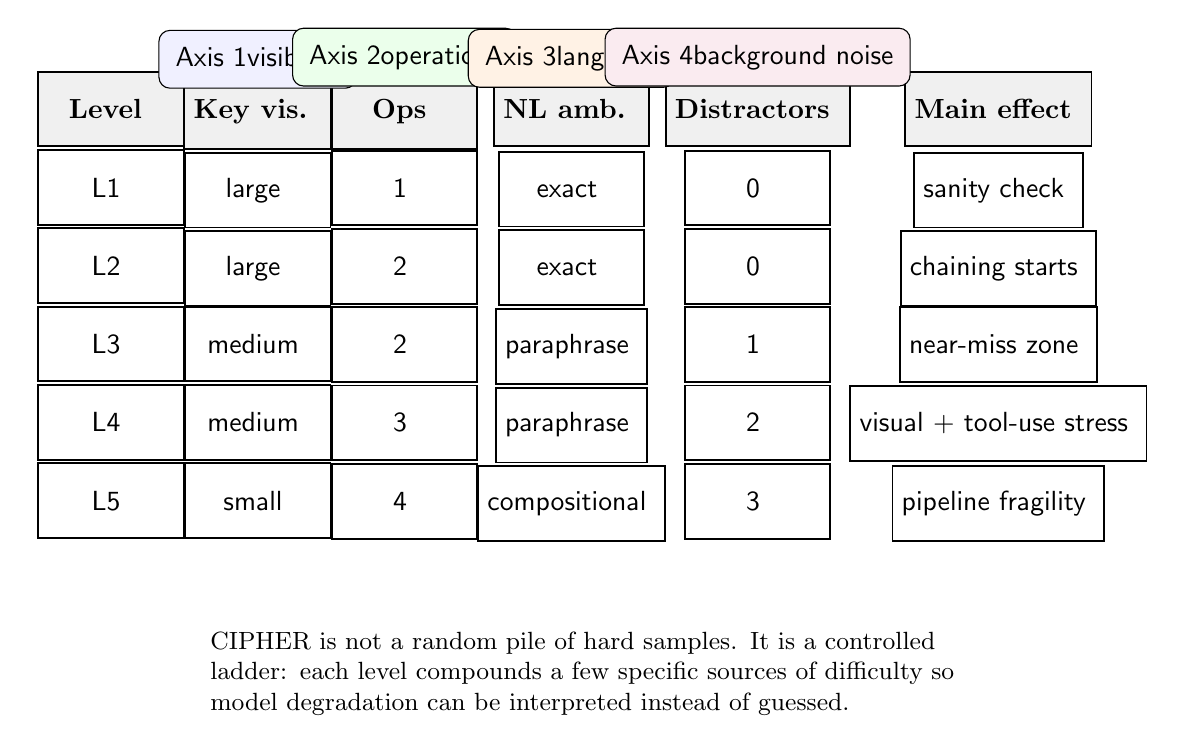
\begin{tikzpicture}[
  font=\sffamily,
  cell/.style={draw, minimum width=1.85cm, minimum height=0.95cm, align=center, line width=0.7pt},
  hdr/.style={cell, fill=gray!12, font=\bfseries},
  note/.style={font=\small, text width=9.7cm, align=left}
]

\matrix[matrix of nodes, nodes in empty cells, row sep=-\pgflinewidth, column sep=-\pgflinewidth] (m) {
|[hdr]| Level & |[hdr]| Key vis. & |[hdr]| Ops & |[hdr]| NL amb. & |[hdr]| Distractors & |[hdr]| Main effect \\
|[cell]| L1 & |[cell]| large & |[cell]| 1 & |[cell]| exact & |[cell]| 0 & |[cell]| sanity check \\
|[cell]| L2 & |[cell]| large & |[cell]| 2 & |[cell]| exact & |[cell]| 0 & |[cell]| chaining starts \\
|[cell]| L3 & |[cell]| medium & |[cell]| 2 & |[cell]| paraphrase & |[cell]| 1 & |[cell]| near-miss zone \\
|[cell]| L4 & |[cell]| medium & |[cell]| 3 & |[cell]| paraphrase & |[cell]| 2 & |[cell]| visual + tool-use stress \\
|[cell]| L5 & |[cell]| small & |[cell]| 4 & |[cell]| compositional & |[cell]| 3 & |[cell]| pipeline fragility \\
};

\node[draw, rounded corners=4pt, fill=blue!6, inner sep=6pt, above=0.8cm of m-2-2] (a1) {Axis 1\\visibility};
\node[draw, rounded corners=4pt, fill=green!8, inner sep=6pt, above=0.8cm of m-2-3] (a2) {Axis 2\\operations};
\node[draw, rounded corners=4pt, fill=orange!10, inner sep=6pt, above=0.8cm of m-2-4] (a3) {Axis 3\\language};
\node[draw, rounded corners=4pt, fill=purple!8, inner sep=6pt, above=0.8cm of m-2-5] (a4) {Axis 4\\background noise};

\node[note, below=0.9cm of m] {
CIPHER is not a random pile of hard samples. It is a controlled ladder: each level compounds a few specific sources of difficulty so model degradation can be interpreted instead of guessed.
};

\end{tikzpicture}
\end{document}
